\newpage
\textbf{\textcolor{MidnightBlue}{4.}}
Decimos que un canal de comunicación entre dos procesos $p_i$ y $p_j$ es \code{FIFO} si los
mensajes se reciben en el mismo orden en el que se envían. Entonces, si el canal \code{NO}
es \code{FIFO}, puede ser que $p_i$ envía primero $M_1$ y después $M_2$, pero $p_j$
reciba primero $M_2$ y después $M_1$.\\

Dados dos procesos que comparten un canal $C$ que no es \code{FIFO}, da un algoritmo que
implemente un canal \code{FIFO} sobre $C$. Tu algoritmo debe tener dos secciones: una sección
{\bf send}, que recibe como entrada un mensaje $M$ a enviarse (el cuál se envía finalmente
por $C$), y una sección {\bf receive}, que recibe un mensaje $M$ de $C$ y lo entrega. De esta
forma, otro algoritmo que esté diseñado para canales \code{FIFO} puede usar tu algoritmo para
enviar y recibir mensajes. Este esquema se puede observar en la figura 2. Argumenta que tu
algoritmo es correcto. Tip: piensa en \code{timestamps} y considera que un mensaje que se
recibe de $C$ no tiene que entregarse inmediatamente.

\begin{center}
    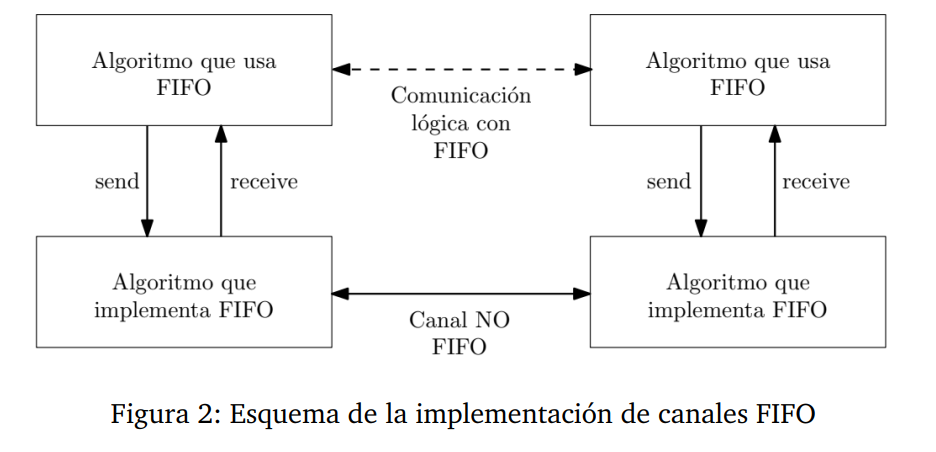
\includegraphics[scale=0.5]{Grapho1.png}
    \end{center}

    % Algoritmo
    \hfill\break
      %%\rule{1\textwidth}{0.2mm}
    \hspace*{.2cm} {\bf Algoritmo:} No\_FIFO.
    \hfill\break
    1. // F. Auxiliar que realiza los registros (locales).
    \hfill\break
    2. record():
    \hfill\break
    3. $\sigma_i\leftarrow$ estado actual de $p_i$
    \hfill\break
    4. //Estado global respecto a $p_i$
    \hfill\break
    5. globalSt $\leftarrow$ rojo \hspace{0.5cm}  // $rojo$ si el estado esta registrado
    \hfill\break
    6. {\bf registra} $\sigma_i$ receive[c\_entrada], {\bf and} sent[c\_salida]
    \hfill\break
    7. {\bf send} lo anterior a $pc$ \hspace{0.5cm}  //Sea $pc$ un proceso controlador.
    \hfill\break
    8.
    \hfill\break
    9. Al inicializarse:
    \hfill\break
    10. {\bf if} $globalSt = verde$ {\bf then} $record()$ {\bf end if}
    \hfill\break
    11.
    \hfill\break
    12. //Seccion receive
    \hfill\break
    13. Al recibir un mensaje $(m)$ $entra\_canal[j]$:
    \hfill\break
    14. $receive[j] \leftarrow receive[j] \cup \{m\}$
    \hfill\break
    15. {\bf if} $(m.color = rojo) \,\,\land (globalSt = verde)$ {\bf then} $record()$ {\bf end if}
    \hfill\break
    16. pasa el mensaje a $p_i$
    \hfill\break
    17.
    \hfill\break
    18. //Seccion send
    \hfill\break
    19. Al enviar un mensaje $(m)$ $sale\_canal[j]$:
    \hfill\break
    20. $m.color \leftarrow globalSt$
    \hfill\break
    21. $sent[k] \leftarrow sent[j] \cup \{m\}$
    \hfill\break

    \newpage
    Cuando el controlador recibe cada $pc_i$ (Nota: $pc$ es un proceso controlador),
    los reúne para obtener la suma de cada uno de los estados de $p_i$. Y la suma de
    los canales $C$, se definirá el estado del canal de $p_j$ $p_i$ como:\\
    $c\_estado(j,i)= sent[i] \,\, and \,\, receive[j]$.\\

    El algoritmo es correcto, ya que de la definición se tiene que $sent[i]$ es el
    conjunto de mensajes enviados por $p_j$ a $p_i$ antes del estado $j$ ($\sigma_j$)
    y también de que $receive[j]$ es el conjunto de mensajes recibidos de $p_i$ a $p_j$
    antes del estado $i$ ($\sigma_i$), que el estado de $c\_estado(j,i)$, registra los
    mensajes que están en translado respecto al par ordenado de los estados
    $(\sigma_j,\sigma_i)$.\\

    Como no se encuentran mensajes perdidos respecto a los estados de manera local registrados,
    por lo que el estado global al final será consistente.
